% !TeX spellcheck = en_US
\documentclass[a4paper, runningheads]{llncs}

% Full page margins
\usepackage{fullpage}

% For language
\usepackage[english]{babel}
\usepackage[utf8]{inputenc}

% For figures
\usepackage{graphicx}
\usepackage{caption}
\usepackage{subcaption}

% For tables
\usepackage[dvipsnames,table,xcdraw]{xcolor}
\usepackage{multirow}
\renewcommand{\arraystretch}{1.2}

% Glossary
\usepackage[acronym]{glossaries}
\makenoidxglossaries

% Acronyms
\newacronym{dl}{DL}{Deep learning}
\newacronym{relu}{ReLU}{Rectified Linear Unit}
\newacronym{ann}{ANN}{artificial neural network}
\newacronym{sisr}{SISR}{single image super-resolution}
\newacronym{hr}{HR}{high resolution}
\newacronym{lr}{LR}{low resolution}
\newacronym{cnn}{CNN}{convolutional neural network}
\newacronym{srcnn}{SRCNN}{Super-Resolution Convolutional Neural Network}
\newacronym{fsrcnn}{FSRCNN}{Fast Super-Resolution Convolutional Neural Network}
\newacronym{ircnn}{IRCNN}{Image Restoration Convolutional Neural Network}
\newacronym{psnr}{PSNR}{Peak Signal to Noise Ratio}
\newacronym{ssim}{SSIM}{structural similarity}
\newacronym{gpu}{GPU}{graphics processing unit}
\newacronym{dncnn}{DnCNN}{Denoising Convolutional Neural Network}
\newacronym{gan}{GAN}{Generative Adversarial Networks}
\newacronym{lapsrn}{LapSRN}{Deep Laplacian Pyramid Super-Resolution Network}
\newacronym{vdsr}{VDSR}{Very Deep Super-Resolution}
\newacronym{espcn}{ESPCN}{Efficient Sub-Pixel Convolutional Neural Network}
\newacronym{edsr}{EDSR}{Enhanced Deep Super-Resolution}
\newacronym{mrf}{MRF}{Markov random fields}
\newacronym{bm3d}{BM3D}{Block-matching and 3D filtering}
\newacronym{ncsr}{NCSR}{Nonlocally Centralized Sparse Representation}
\newacronym{hqs}{HQS}{Half Quadratic Splitting}
\newacronym{tnrd}{TRND}{Trainable Nonlinear Reaction Diffusion}
\newacronym{deepam}{DeepAM}{Deeply aggregated Alternating Minimization}
\newacronym{prelu}{PReLU}{Parametric Rectified Linear Unit}
\newacronym{nhwc}{NHWC}{number of samples, height, width, channels}
\newacronym{nchw}{NCHW}{number of samples, channels, height, width}
\newacronym{rgb}{RGB}{Red, Green, Blue}
\newacronym{ycbcr}{YCbCr}{$YC_bC_r$: $Y$, luma component, $C_b$, blue-difference component, $C_r$, red-difference component}
\newacronym{mse}{MSE}{Mean Squared Error}
\newacronym{sgd}{SGD}{stochastic gradient descent}
\newacronym{os}{OS}{operative system}


% For bibliography
\usepackage[backend=biber]{biblatex}
\usepackage{csquotes}
\addbibresource{references.bib}

% For links
\usepackage{hyperref}
\usepackage{cleveref}
\hypersetup {
	linkcolor  = MidnightBlue,
	citecolor  = MidnightBlue,
	urlcolor   = MidnightBlue,
	colorlinks = true,
}

\begin{document}

	% Title
	\title{Single Image Super-Resolution and Denoising using Convolutional Neural Networks}
	\author{Guillermo Ruiz Álvarez}
	\institute{University of Málaga - \email{grabmct@uma.es}}
	
	\maketitle
	
	\abstract{We analyze the behavior of applying two well-known deep learning methods for single image super-resolution and image denoising, namely FSRCNN \cite{FSRCNN} and IRCNN \cite{IRCNN}, in different order to evaluate their combined capability to restore low resolution images with presence of noise. In order not to limit the case study to a single type of noise, Gaussian noise, Poisson noise, salt-and-pepper noise and uniform noise are applied to down-scaled images in order to construct the degraded images to be restored. As a result, we find that applying IRCNN before super-resolving the images with FSRCNN shows better results than using the networks in the opposite order for all types of noise. We also compare the quality achieved by using these deep learning methods in combination with other traditional algorithms: bicubic interpolation for super-resolution and median and wavelet filtering for image denoising. Our experimental results show that FSRCNN and IRCNN achieve better restoration quality than when the selected traditional methods are applied.
	
	\keywords{Single Image Super-Resolution, Image Denoising, Image Restoration, Convolutional Neural Networks.}\\~
	
	\textbf{Supervisors:} Ezequiel López Rubio, Rafael Marcos Luque Baena.
	
	\section{Introduction}

\Gls{sisr} and image denoising are two common low-level tasks in the field of computer vision. \Gls{sisr} is a classical problem that aims at recovering a \gls{hr} image from a given \gls{lr} version of the same image. This problem is ill-posed because a given \gls{lr} input can correspond to multiple \gls{hr} solutions and therefore reliable prior information is usually required to constraint the solution space \cite{DBLP:SISR} \cite{SRCNN} \cite{DBLP:DEEPSISR}. On the other hand, image denoising is the process of estimating the clean and original version of an image given a noisy input.

\gls{sisr} and image denoising have received increasing attention by researches due to their multiple applications in the field of computer vision. The various methods that have been developed to tackle these two tasks can be broadly classified into two groups: traditional and deep learning methods. Deep learning methods, and more specifically those using \glspl{cnn}, have achieved promising results in terms of performance and restoration of quality for both tasks \cite{DBLP:DEEPNR} \cite{DBLP:DEEPSISR}.

However, applying \gls{sisr} and denoising methods in conjunction might produce undesired results if the presence of noise in the \gls{lr} images affects the super-resolution task or, likewise, if the result of denoising an input image degrades the quality of the super-resolution step. Therefore, this study aims at analyzing which is the most efficient process to produce \gls{hr} images given \gls{lr} inputs with presence of different types of noise using deep learning methods based on \glspl{cnn}. For this study, we have selected Gaussian noise, Poisson noise, salt-and-pepper noise and uniform noise to be applied to down-scaled versions of the images to be restored.

Among all the deep learning methods for \gls{sisr} and image denoising, experimental results using the \gls{fsrcnn} \cite{FSRCNN} and the \gls{ircnn} \cite{IRCNN} have demonstrated promising results and high performance in their implementations in \glspl{gpu} and therefore we have selected them in order to perform the case study.

For the analysis, both networks have been trained using the same training and validation datasets (BSD200 \cite{BSDS}, General100 \cite{FSRCNN} and T91 \cite{T91}) and have been evaluated with Set5 \cite{SET5} and Set14 \cite{SET14} using \gls{psnr} and \gls{ssim} as quality metrics.

Furthermore, we have also selected traditional methods for both super-resolution and image denoising in order to compare the efficiency of applying traditional and deep learning methods to tackle these low-level computer vision tasks. More specifically, we have used bicubic interpolation for \gls{sisr} and median and wavelet filtering for image denoising.

The contribution of this study can be summarized as follows:
\begin{itemize}
	\item We perform an analysis on the application of  \gls{fsrcnn} and \gls{ircnn} in conjunction for tackling \gls{sisr} and image denoising tasks in order to restore \gls{lr} images with presence of different types of noise.
	\item We provide an evaluation comparing traditional and deep learning \gls{sisr} and image denoising methods on two popular testing datasets (Set5, Set14).
	\item We provide a Keras \cite{KERAS} implementation of \gls{fsrcnn} and \gls{ircnn} that can be used for both training and inference.
	\item We discuss possible future directions for \gls{sisr}+denoising research studies.
\end{itemize}

The remainder of this study is structured as follows: Section \ref{sec:background}, introduces the concepts of deep learning, \glspl{cnn}, \gls{sisr} and noise reduction. Section \ref{sec:deep_learning} summarizes the state-of-the-art \glspl{cnn} and other deep learning methods for \gls{sisr} and image denoising. Besides, it provides an overview of the structure of the two \glspl{cnn} used in this study: \gls{fsrcnn} and \gls{ircnn}. Section \ref{sec:experimental_design} describes the implementation details concerning the training, validation and test datasets, the data pre-processing and the training and inference strategies for the experiments that have been carried out. In Section \ref{sec:experiments}, we discuss the results of these experiments and provide a comparison with traditional methods for \gls{sisr} and denoising. Section \ref{sec:conclusions} presents the conclusions of this study and provides insight into possible future research directions.
	\section{Background}

	% !TeX spellcheck = en_US
\section{Deep Learning for SISR and noise reduction}\label{sec:deep_learning}

\subsection{Deep Learning for Single Image Super-Resolution}
Recently, deep learning methods for \gls{sisr} have demonstrated promising performance and accuracy compared to conventional \gls{sisr} algorithms. Before \gls{srcnn} \cite{SRCNN} was presented, which is the pioneer work in the field, Yang et al. \cite{SISRBENCH} categorized \gls{sisr} algorithms in 4 groups based on the image prior:
\begin{itemize}
	\item Prediction models, that apply a predefined mathematical formula to generate \gls{hr} outputs without training data. Bilinear, bicubic and Lanczos interpolation methods are examples of algorithms in this group.
	\item Edge based methods, that learn priors from edge features in order to predict \gls{hr} images from \gls{lr} images.
	\item Image statistical methods, that use statistical properties of the images as priors to reconstruct the \gls{hr} images.
	\item Patch based methods, that learn mapping functions from sets of paired \gls{lr} and \gls{hr} training images.
\end{itemize}

With the publication of \gls{srcnn} \cite{SRCNN}, deep learning methods can be added to this taxonomy. Within this category, multiple methods using different kinds of neural network have been developed. 

Kim et al. proposed \gls{vdsr} \cite{VDSR}, that uses similar structure as \gls{srcnn} but using a deeper network.

\gls{espcn} \cite{ESPCN} was proposed by Shi et al to make \gls{srcnn} more efficient. This network performs the feature extraction in the \gls{lr} space in order to consume less computational resources. Once the extraction is done, it uses a sub-pixel convolution in order to reconstruct the \gls{hr} image.

Dong et al. designed \gls{fsrcnn} \cite{FSRCNN} by accelerating \gls{srcnn} \cite{SRCNN} in multiple steps. First, the last convolution layer of \gls{srcnn} was replaced by a deconvolution layer, eliminating the need for using bicubic interpolation on the input \gls{lr} image. Second, the non-linear mapping layer was replaced by a shrinking layer, 4 non-linear mapping layer and an expanding layer, increasing the number of layers but reducing the number of parameters.

Residual networks have also been used for the \gls{sisr} task \cite{EDSR}\cite{REDNET}. These networks use skip connections to jump over some of their layers in order to tackle the problem of gradient vanishing, allowing to design very deep networks.

Lai et al. proposed \gls{lapsrn} \cite{LAPSRN}\cite{LAPSRN2}, based on a Laplacian pyramid framework, that progressively reconstructs the sub-band residuals from its feature extraction branch in order to obtain the \gls{hr} images. 

Some image denoisers, such as \gls{ircnn} \cite{IRCNN} and \gls{dncnn} \cite{DNCNN} also address the problem of \gls{sisr}. These methods model the image degradation in the \gls{sisr} problem by taking the noise as the difference between the \gls{hr} image and the bicubic upsampling of the \gls{lr} image.
 
\gls{gan} have also been used for \gls{sisr} \cite{SRGAN}. In these models, two neural networks contest with each other, in the context of game theory, in order to solve the super-resolution problem. The generative network generates output data by super-resolving \gls{lr} images and the discriminative network evaluates them. The objective of the discriminative network is to distinguish between real \gls{hr} images and super-resolved images while the generative network tries to increase its error rate.

Anwar et al. \cite{DBLP:SISR} proposed a taxonomy that categorizes deep learning methods for \gls{sisr} into 9 different groups according to their model designs, namely, linear networks, residual networks, recursive networks, progressive reconstruction designs, densely connected networks, multi-branch designs, attention based networks, multiple degradation handling networks and \gls{gan} models.

\subsection{Deep Learning for Image Denoising}
Image denoising is another important task in computer vision applications. Over the past years, multiple methods for modeling image priors, such as \gls{mrf} \cite{MRF}, \gls{bm3d} \cite{BM3D} and \gls{ncsr} \cite{NCSR}, have been proposed in order to tackle this problem. However, the mentioned methods have shown high computational cost and they also need to have their parameters manually chosen in order to improve performance \cite{DBLP:DEEPNR}. Multiple methods have been proposed to solve these problems. 

In \cite{TNRD}, Chen et al. presented a  \gls{tnrd} model in which the filters and the influence functions can be learned from the training data., 

In \cite{DEEPAM}, Kim et al. proposed \gls{deepam}, which learns a regularizer via deep aggregation in order to solve multiple image restoration tasks, including single image denoising.  

Zhang et al. proposed \gls{dncnn} \cite{DNCNN}, which uses residual learning and batch normalization in order to speed up the training process and boost the denoising performance.

Zhang et al. also proposed \gls{ircnn} \cite{IRCNN}, which is a \gls{cnn} based image denoiser that can be used for several low-level computer vision tasks such as \gls{sisr} or deblurring. \gls{ircnn} uses \gls{hqs} to show that a \gls{cnn} based denoiser prior can be plugged as a modular part of model-based optimization methods in order to solve multiple inverse problems.

In \cite{DILATED}, Wang et al. present a dilated residual \gls{cnn} for Gaussian image denoising in which the receptive field is enlarged by adopting dilated convolution.

\subsection{FSRCNN and IRCNN}
In this subsection, we review the structure of the two \glspl{cnn} used in this study: \gls{fsrcnn} and \gls{ircnn}.

\subsubsection{FSRCNN} The structure of \gls{fsrcnn} is composed of 5 different layers, 4 convolution layers and a deconvolution layer:
\begin{itemize}
	\item \textbf{Feature extraction}. This operation extracts overlapping patches from the \gls{lr} input by convolving them with a set of $d$ filters that represent each patch as a high dimensional feature vector. The size of the filters proposed by the authors for this layer is $5$. On the other hand, the input number of channels is $1$.
	\item \textbf{Shrinking}. A shrinking layer is added after the feature extraction in order to reduce the \gls{lr} feature dimension by convolving the \gls{lr} features with $s$ filters of size $1$. With this filter size, linear combinations applied in the  \gls{lr} feature space reduce its dimension from $d$ to $s$, decreasing as well the number of parameters and therefore the computational cost.
	\item \textbf{Non-linear mapping}. 
	\item Expanding:
	\item Deconvolution:
\end{itemize}

Following the notation proposed in \cite{fsrcnn}, we denote the convolution layers as $Conv(f_i, n_i, c_i)$ and the deconvolution layer as $DeConv(f_i, n_i, c_i)$ where $f_i$ is the size of the filter, $n_i$ is the number of filters and $c_i$ is the number of channels in the $i-th$ layer.

\subsubsection{IRCNN}

	% !TeX spellcheck = en_US
\section{Experimental Design}\label{sec:experimental_design}

In this section, we present the image datasets used for the training, validation and test steps, we expose the details of our implementation of both \glspl{cnn}, we show how the images are pre-processed before the training and we described the followed training strategies and set of experiments.

\subsection{Training, Validation and Test datasets}

For training and validation, BSD200 \cite{BSDS}, General100 \cite{FSRCNN} and T91 \cite{T91} datasets have been used, bringing the total of images to 391. A 10\% of these images have been randomly chosen for validation, therefore, the training set has 352 images and the validation set, 39.

Set5 \cite{SET5} and Set14 \cite{SET14} have been used for the test stage, making a total of 19 images.

The same training, validation and test datasets have been used for both \gls{fsrcnn} and \gls{ircnn}. 

\subsection{Implemented \glspl{cnn}}
For this study, we have used our own implementation of \gls{fsrcnn} and \gls{ircnn} using Keras \cite{KERAS} in order to use the same deep learning framework for both networks.

Both of them use a sequential model in order to stack bi-dimensional convolution (or deconvolution) layers. All the layers use the format \gls{nhwc}.

In order to deal with the boundary artifacts produced by the convolution operation, zero padding has been adopted in all layers according to the filter size.

For FSRCNN, the filters are initialized with variance scaling for all the convolution layers and with a Gaussian distribution with zero mean and standard deviation 0.001 for the deconvolution layer. Furthermore, for the mapping depth, the LR feature dimension and the number of shrinking filters, we have used, $m=4$, $d=48$ and $s=16$, respectively, since in \cite{FSRCNN}, these settings show outstanding \gls{psnr} results compared to the rest of investigated settings.

For IRCNN, glorot uniform initializer \cite{XAVIER} is used to initialize the filters of all the convolution layers.

All the implementation details of the \glspl{cnn} and the datasets used can be found at \href{https://github.com/guillermoruizalv/restore}{https://github.com/\\guillermoruizalv/restore}.

\subsection{Image pre-processing}
Before being used as input of the neural networks, the 391 images used for training and validation are pre-processed using some common and some model-dependent steps:
\begin{itemize}
	\item First, since we are using \gls{rgb} images with true color (24 bits, 8-bits per channel), all the images are loaded as 3-dimensional matrices using uint8 (unsigned 8-bit integer) data type.
	
	Only for \gls{fsrcnn}, the images are converted from \gls{rgb} to \gls{ycbcr}. Specifically, the $Y$ component is super-resolved by the network and the blue-difference and red-difference components are upscaled using bicubic interpolation.
	
	\item Once the images are loaded, they are scaled to $[0,1]$ range and transformed to float64 (double precision floating-point format). 
	
	\item The resulting images are cropped into $32\times32$ sub-patches using a stride of size $16$ in order not to lose the information between adjacent patches. The remaining pixels are discarded.
\end{itemize}

This process results in 170293 sub-patches for training and 20705 sub-patches for validation.

A last pre-processing step is applied to the training and validation images depending on the model that is going to be trained.
\begin{itemize}
	\item For \gls{fsrcnn}, Lanczos interpolation is used in order to downscale the data using a scale factor of 2. Before downscaling, if the number of rows or the number of columns is not even, the bottom-most row or the right-most column are discarded, respectively. This is done so that when \gls{fsrcnn} upscales the image, the output of the network has the same dimensions as the labels.
	\item For \gls{ircnn}, random noise is added to the patches using the following parameters:
	\begin{itemize}
		\item The noise method to be applied is chosen randomly from Gaussian noise, Poisson noise, salt-and-pepper noise and uniform noise using the same probability.
		\item If Gaussian noise is selected, $\mu$ is set to 0 and $\sigma$ takes a random value from the range $[0.05, 0.15]$.
		\item If Poisson noise is selected, input pixel values are interpreted as means of Poisson distributions scaled up by $2^8$.
		\item If salt-and-pepper noise or uniform noise is selected, the noise ratio takes a random value from the range $[0.05, 0.20]$.
	\end{itemize}
\end{itemize}

\subsection{Training hardware, strategy and results}
\paragraph{Training hardware}
The training has been carried out in a server running Ubuntu 18.04 LTS with a Nvidia Geforce GTX 1060 with compute capability of $6.1$. Most of the development has been done in a different machine with the same \gls{os} and a Nvidia Geforce GT 730M with compute capability of $3.5$.

\paragraph{Training strategy}
The training strategy adopted for \gls{fsrcnn} and \gls{ircnn} is common for both cases except for the used learning rates.

\begin{itemize}
	\item \textbf{Image loading and memory management}. Due to the big amount of data used for the training, the training and validation images have been loaded dynamically so that the pre-processing held a maximum of 64 images at a time. 
	
	This allowed us to consume less memory resources on both the machine and the \gls{gpu} that have been used for the experiments, given their memory limitations. Consequently, the training performance was slightly reduced since for each epoch, the training images had to be loaded multiple times.
	
	\item \textbf{Batch size}. A batch size of $256$ samples has been selected, producing $666$ batches for the training images and $81$ batches for the validation images.
	
	\item \textbf{Reproducibility and number of threads}. In order to be able to reproduce the noise generation, we set the random seed of the \textit{numpy.random} module to $1$ at the beginning of each epoch. 
	
	However, unlike the \textit{random} module, \textit{numpy.random} is not thread-safe. For this reason, we have set the number of threads to $1$ slightly losing some performance when generating the training images but having the ability to generate equal noisy sub-patches for each epoch.
	
	\item \textbf{Loss function}. The loss function used in both cases is \gls{mse}:
	$$MSE = \frac{1}{n}\sum_{i=0}^{n}\left(Y_{pred}-Y_{true}\right)$$
	where $Y_{pred}$ is the predicted result of the network and $Y_{true}$ is the value of the label.
	\item \textbf{Optimizer}. The Adam optimizer \cite{ADAM} has been used for both models. Although \gls{sgd} is proposed in \cite{FSRCNN} for training \gls{fsrcnn}, we empirically found that the Adam optimizer offered better training performance.
	
	The selected learning rates for this optimizer are:
	\begin{itemize}
		\item For \gls{fsrcnn}, an initial learning rate of $10^{-3}$ is used. This value is reduced to a minimum of $10^{-4}$ using a patience of $10$ on the validation set. This means that the learning rate is reduced when the validation loss has stopped improving for $10$ epochs in a row.
		\item For \gls{ircnn}, an initial learning rate of $10^{-4}$ is used. For this model, the patience is also set to $10$, after which the learning rate is reduced to a minimum of $10^{-5}$. 
		
		Our initial experiments with \gls{ircnn} were using the same learning rate values as \gls{fsrcnn}. However, we noticed that the model stopped learning very early and that the loss function on the training and validation datasets was oscillating over the training epochs. For this reason, the learning rate values were reduced with a scale of $0.1$, improving the training performance.
	\end{itemize}
    \item \textbf{Early stopping}. Instead of setting a specific number of training epochs, we monitor the performance of the models and we use early stopping on the validation loss with a patience of $25$. This means that if the validation loss has not improved after 25 epochs in a row, the training will be automatically stopped.
    
    The reason why we use early stopping instead of a given number of epochs is to avoid over-training,   reduce over-fitting and improve the generalization of the \glspl{cnn}.

\end{itemize}

\paragraph{Training results}
Using this training strategy, we have had the following training results:
\begin{itemize}
	\item \gls{fsrcnn} was trained for 1092 epochs during approximately one day, reaching a minimum validation loss value of $0.0011$.
	\item \gls{ircnn} was trained for 891 epochs during approximately four days, reaching a minimum validation loss value of $5.0165\times10^{-4}$.
\end{itemize}

The learning curves of both \glspl{cnn} are presented in Figure \ref{fig:training}. We can observe that, for \gls{ircnn}, the validation loss is oscillating around epoch $50$. After $10$ epochs, the learning rate is reduced with a scale factor of $0.1$ and the validation loss continues decreasing.

In earlier experiments, the training was stopping at this stage after 25 epochs before we reduced the learning rate to a minimum of $10^{-5}$.

\begin{figure}[h]
	\centering
	\begin{subfigure}{0.49\textwidth}
		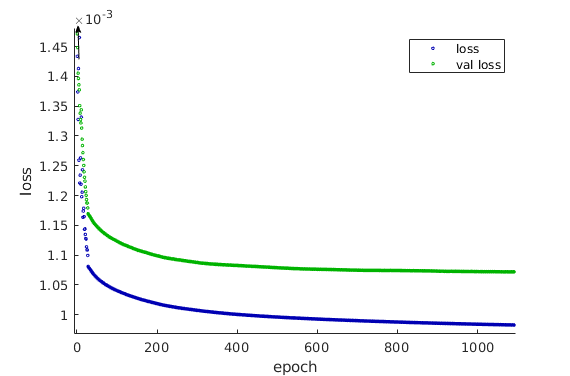
\includegraphics[width=\textwidth]{images/fsrcnn_train.png}
		\caption{\gls{fsrcnn}}
	\end{subfigure}
	\begin{subfigure}{0.49\textwidth}
		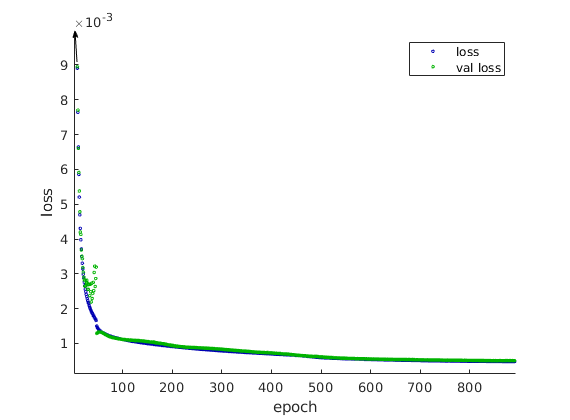
\includegraphics[width=\textwidth]{images/ircnn_train.png}
		\caption{\gls{ircnn}}
	\end{subfigure}
	\caption{\glspl{cnn} learning curves.}
	\label{fig:training}
\end{figure}

\subsection{Set of experiments}
We have carried out the following set of experiments using Set5 \cite{SET5} and Set14 \cite{SET14} as test datasets:
\begin{itemize}
	\item \textbf{Experiment 1.1}: Evaluation of \gls{fsrcnn} $+$ \gls{ircnn} on Set5 and Set14.
	\item \textbf{Experiment 1.2}: Evaluation of \gls{ircnn} $+$ \gls{fsrcnn} on Set5 and Set14.
\end{itemize}

The aim of these two experiments is to get to know which combination performs better on the given noisy images.

Apart from these and given their results, we also perform the following experiments in order to evaluate the performance of the deep learning methods compared to the selected traditional methods. This set of experiments use a deep learning method and a traditional method for either \gls{sisr} or image denoising:
\begin{itemize}
	\item \textbf{Experiment 2.1}: Evaluation of \gls{ircnn} $+$ bicubic interpolation.
	\item \textbf{Experiment 2.2}: Evaluation of wavelet denoiser $+$ \gls{fsrcnn}.
	\item \textbf{Experiment 2.3}: Evaluation of median filter $+$ \gls{fsrcnn}.
\end{itemize}

Finally, the following set of experiments is carried out to have a benchmark based purely on traditional algorithms:
\begin{itemize}
\item \textbf{Experiment 3.1}:  Evaluation of wavelet denoiser $+$ bicubic interpolation.
\item \textbf{Experiment 3.2}:  Evaluation of median filter $+$ bicubic interpolation.
\end{itemize}
All these experiments are carried out using \gls{psnr} and \gls{ssim} as quality metrics.
	% !TeX spellcheck = en_US
\section{Experiments}\label{sec:experiments}
In this section, we present the results of all the experiments described before in this document.  

All the evaluations are performed using Set5 \cite{SET5} and Set14 \cite{SET14}, which are degraded by applying the following algorithms in order to obtain the \gls{lr} images:

\begin{itemize}
\item First, all the images in Set5 and Set14 are downscaled using Lanczos interpolation with a scale factor of 2. 
\item Second, we apply one of the following noise types varying the noise parameters in order to enlarge the test set:
\begin{itemize}
	\item Gaussian noise is applied using $\mu=0$ and $\sigma = 0.05, \sigma = 0.10$ or $\sigma = 0.15$.
	\item Poisson noise is applied using input pixels values as means of Poisson distributions scaled up by $2^8$.
	\item Salt-and-pepper and uniform noise is applied using noise ratios of $0.05, 0.10, 0.15$ and $0.20$.
\end{itemize}
\end{itemize}

After applying these filters with the respective parameters variation, we end up having 12 sets of 19 images, making a total of 228 \gls{lr} images, which correspond to the 19 \gls{hr} images of Set5 and Set14. Figure \ref{fig:exp0} shows some examples of this processing applied to an image taken from Set5.

\begin{figure}
	\centering
	\begin{subfigure}{0.24\textwidth}
		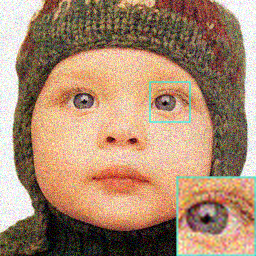
\includegraphics[width=\textwidth]{images/exp0.1/gaussian0.png}
		\caption{Gaussian, $\sigma=0.1$}
	\end{subfigure}
	\begin{subfigure}{0.24\textwidth}
		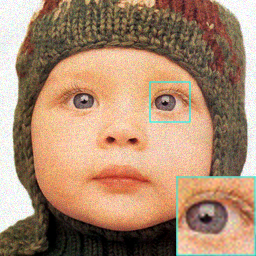
\includegraphics[width=\textwidth]{images/exp0.1/poisson0.png}
		\caption{Poisson}
	\end{subfigure}
	\begin{subfigure}{0.24\textwidth}
		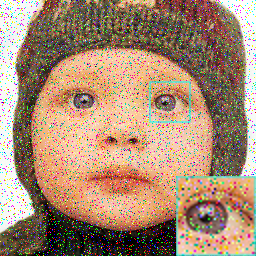
\includegraphics[width=\textwidth]{images/exp0.1/salt0.png}
		\caption{S\&P, $r=0.1$}
	\end{subfigure}
	\begin{subfigure}{0.24\textwidth}
		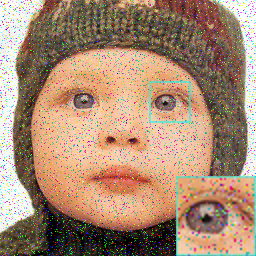
\includegraphics[width=\textwidth]{images/exp0.1/uniform0.png}
		\caption{Uniform, $r=0.1$}
	\end{subfigure}
\caption{The image ``baby'' from Set5, degraded using downscaling with a factor of 2 and different types of noise.}
\label{fig:exp0}
\end{figure}

In order to generate the noisy images, we have used custom functions that can be found along with the implementation of the \glspl{cnn} and the datasets. In these functions, the random seed is initially set to 0. The same 228 images are used for all the experiments.

For the experiments that make use of median filter and wavelet denoiser, we apply the \textsc{matlab} functions \texttt{medfilt2()} and \texttt{wdenoise2()}.

In order to perform the evaluation of the quality metrics, the \textsc{matlab} functions \texttt{psnr()} and \texttt{ssim()} are used.

\newpage\subsection{Experiment 1.1}
In this experiment, we evaluate \gls{fsrcnn} $+$ \gls{ircnn} on our set of 228 \gls{lr} images. The results of this experiment are presented in Table \ref{tab:experiment11}.

\begin{table}[h]
	\centering
	\begin{tabular}{|l|l|r|r|r|r|}
		\hline
		\rowcolor[HTML]{EFEFEF} 
		\multicolumn{1}{|c|}{\cellcolor[HTML]{EFEFEF}\textbf{Noise}} & \textbf{Parameters} & \multicolumn{1}{c|}{\cellcolor[HTML]{EFEFEF}\textbf{Set5 \gls{psnr} (dB)}} & \multicolumn{1}{c|}{\cellcolor[HTML]{EFEFEF}\textbf{Set5 \gls{ssim}}} & \multicolumn{1}{c|}{\cellcolor[HTML]{EFEFEF}\textbf{Set14 \gls{psnr} (dB)}} & \multicolumn{1}{c|}{\cellcolor[HTML]{EFEFEF}\textbf{Set14 \gls{ssim}}} \\ \hline
		\rowcolor[HTML]{FFFFFF} 
		\cellcolor[HTML]{EFEFEF} & $\mu=0, \sigma=0.05$ & 26.6621 & 0.8639 & 25.1018 & 0.8065 \\
		\rowcolor[HTML]{EFEFEF} 
		\cellcolor[HTML]{EFEFEF} & $\mu=0, \sigma=0.10$ & 21.5502 & 0.7024 & 20.6851 & 0.6294 \\
		\rowcolor[HTML]{FFFFFF} 
		\multirow{-3}{*}{\cellcolor[HTML]{EFEFEF}Gaussian} & $\mu=0, \sigma=0.15$ & 18.4371 & 0.5669 & 17.7753 & 0.4954 \\
		\rowcolor[HTML]{EFEFEF} 
		Poisson & $peak=2^8$ & 27.9000 & 0.9074 & 25.9664 & 0.8401 \\
		\rowcolor[HTML]{FFFFFF} 
		\cellcolor[HTML]{EFEFEF} & $r=0.05$ & 22.1321 & 0.7678 & 21.1879 & 0.6994 \\
		\rowcolor[HTML]{EFEFEF} 
		\cellcolor[HTML]{EFEFEF} & $r=0.10$ & 18.6522 & 0.6218 & 18.0292 & 0.5487 \\
		\rowcolor[HTML]{FFFFFF} 
		\cellcolor[HTML]{EFEFEF} & $r=0.15$ & 16.4730 & 0.5141 & 16.0007 & 0.4431 \\
		\rowcolor[HTML]{EFEFEF} 
		\multirow{-4}{*}{\cellcolor[HTML]{EFEFEF}Salt-and-pepper} & $r=0.20$ & 14.9244 & 0.4320 & 14.5495 & 0.3670 \\
		\rowcolor[HTML]{FFFFFF} 
		\cellcolor[HTML]{EFEFEF} & $r=0.05$ & 24.3520 & 0.8135 & 23.4238 & 0.7688 \\
		\rowcolor[HTML]{EFEFEF} 
		\cellcolor[HTML]{EFEFEF} & $r=0.10$ & 20.9578 & 0.7032 & 20.5673 & 0.6542 \\
		\rowcolor[HTML]{FFFFFF} 
		\cellcolor[HTML]{EFEFEF} & $r=0.15$ & 18.7674 & 0.6155 & 18.6073 & 0.5642 \\
		\rowcolor[HTML]{EFEFEF} 
		\multirow{-4}{*}{\cellcolor[HTML]{EFEFEF}Uniform} & $r=0.20$ & 17.1090 & 0.5410 & 17.1459 & 0.4914 \\
		\rowcolor[HTML]{FFFFFF} 
		\textbf{All} &  & \textbf{20.6598} & \textbf{0.6708} & \textbf{19.9200} & \textbf{0.6090}\\\hline
	\end{tabular}
	\caption{\gls{psnr} and \gls{ssim} results for the Experiment 1.1}
	\label{tab:experiment11}
\end{table}

In the table, we can see quite low values of \gls{psnr} and \gls{ssim} for both Set5 and Set14. In fact, if we visually inspect the results, we can observe that the images present a large amount of noise for all the cases. This is shown in Figure \ref{fig:exp1.1}, that exposes the results of restoring the downscaled, noisy images of Figure \ref{fig:exp0} using \gls{fsrcnn} $+$ \gls{ircnn}.

\begin{figure}
	\centering
	\begin{subfigure}{0.24\textwidth}
		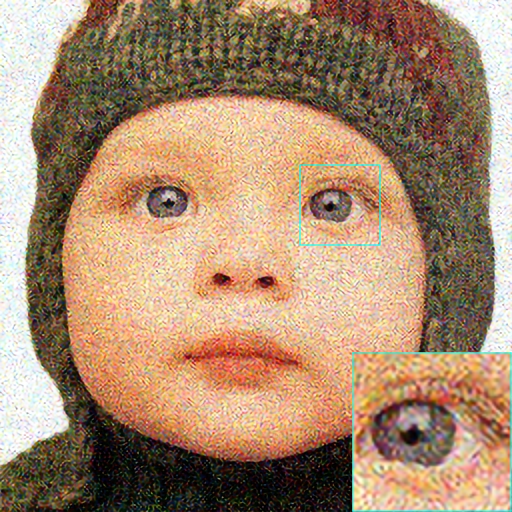
\includegraphics[width=\textwidth]{images/exp1.1/gaussian.png}
		\caption{Gaussian restored}
	\end{subfigure}
	\begin{subfigure}{0.24\textwidth}
		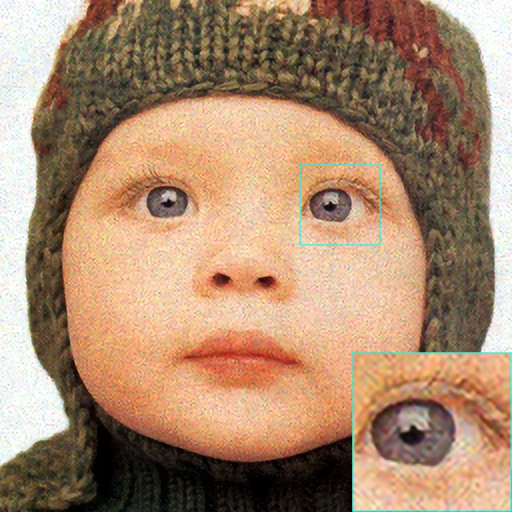
\includegraphics[width=\textwidth]{images/exp1.1/poisson.png}
		\caption{Poisson restored}
	\end{subfigure}
	\begin{subfigure}{0.24\textwidth}
		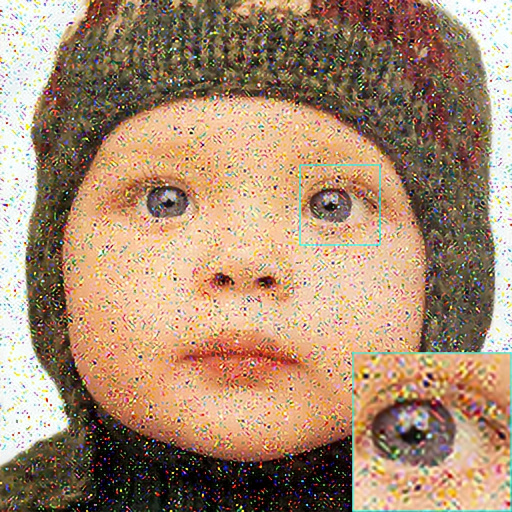
\includegraphics[width=\textwidth]{images/exp1.1/salt.png}
		\caption{S\&P restored}
	\end{subfigure}
	\begin{subfigure}{0.24\textwidth}
		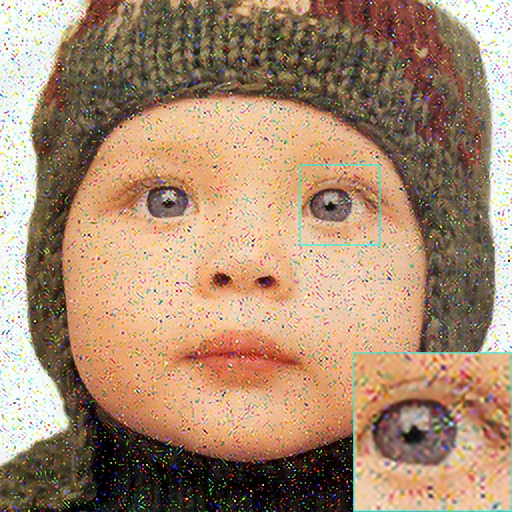
\includegraphics[width=\textwidth]{images/exp1.1/uniform.png}
		\caption{Uniform restored}
	\end{subfigure}
	\caption{Experiment 1.1: restoration using \gls{fsrcnn} $+$ \gls{ircnn}}
	\label{fig:exp1.1}
\end{figure}

In Figure \ref{fig:exp1.1}, we can see that by applying the networks in this order, we cannot remove the noise of the images properly. Instead, \gls{fsrcnn} tries to super-resolve the noise pixels, mixing up the good information of the image with them. Once the image is super-resolved, \gls{ircnn} tries to remove the noise. However, in this case, the resulting noise is a super-resolved version of the original applied noise, and therefore, the network is not capable of detecting the residual part of the image.

This effect repeats for all the images in both Set5 and Set14 and for all noise types. As a consequence, we can observe low \gls{psnr} and \gls{ssim} values in Table \ref{tab:experiment11}.

The results of this experiment shows us that \gls{fsrcnn} $+$ \gls{ircnn} will produce low quality results and that it is not appropriate to super-resolve and denoise our \gls{lr} images.

\newpage\subsection{Experiment 1.2}
In this experiment, we reverse the order of the networks from the previous experiment and evaluate instead the results of applying \gls{ircnn} $+$ \gls{fsrcnn} to our set of \gls{lr} images. Table \ref{tab:experiment12} shows the results of the quality metrics for this experiment. 

\begin{table}[]
	\centering
	\begin{tabular}{|l|l|r|r|r|r|}
		\hline
		\rowcolor[HTML]{EFEFEF} 
		\multicolumn{1}{|c|}{\cellcolor[HTML]{EFEFEF}\textbf{Noise}} & \textbf{Parameters} & \multicolumn{1}{c|}{\cellcolor[HTML]{EFEFEF}\textbf{Set5 \gls{psnr}}} & \multicolumn{1}{c|}{\cellcolor[HTML]{EFEFEF}\textbf{Set5 \gls{ssim}}} & \multicolumn{1}{c|}{\cellcolor[HTML]{EFEFEF}\textbf{Set14 \gls{psnr} (dB)}} & \multicolumn{1}{c|}{\cellcolor[HTML]{EFEFEF}\textbf{Set14 \gls{ssim}}} \\ \hline
		\rowcolor[HTML]{FFFFFF} 
		\cellcolor[HTML]{EFEFEF} & $\mu=0, \sigma=0.05$ & 29.4125 & 0.9055 & 27.1441 & 0.8704 \\
		\rowcolor[HTML]{EFEFEF} 
		\cellcolor[HTML]{EFEFEF} & $\mu=0, \sigma=0.10$ & 27.3907 & 0.8825 & 25.6060 & 0.8255 \\
		\rowcolor[HTML]{FFFFFF} 
		\multirow{-3}{*}{\cellcolor[HTML]{EFEFEF}Gaussian} & $\mu=0, \sigma=0.15$ & 26.0656 & 0.8709 & 24.4851 & 0.7896 \\
		\rowcolor[HTML]{EFEFEF} 
		Poisson & $peak=2^8$ & 30.1634 & 0.9314 & 27.5250 & 0.8855 \\
		\rowcolor[HTML]{FFFFFF} 
		\cellcolor[HTML]{EFEFEF} & $r=0.05$ & 32.3303 & 0.9585 & 28.8342 & 0.9176 \\
		\rowcolor[HTML]{EFEFEF} 
		\cellcolor[HTML]{EFEFEF} & $r=0.10$ & 31.8659 & 0.9498 & 28.5673 & 0.9119 \\
		\rowcolor[HTML]{FFFFFF} 
		\cellcolor[HTML]{EFEFEF} & $r=0.15$ & 31.3457 & 0.9453 & 28.2604 & 0.9067 \\
		\rowcolor[HTML]{EFEFEF} 
		\multirow{-4}{*}{\cellcolor[HTML]{EFEFEF}Salt-and-pepper} & $r=0.20$ & 30.6621 & 0.9395 & 27.8548 & 0.8990 \\
		\rowcolor[HTML]{FFFFFF} 
		\cellcolor[HTML]{EFEFEF} & $r=0.05$ & 32.2225 & 0.9559 & 28.7999 & 0.9160 \\
		\rowcolor[HTML]{EFEFEF} 
		\cellcolor[HTML]{EFEFEF} & $r=0.10$ & 31.5749 & 0.9459 & 28.4277 & 0.9089 \\
		\rowcolor[HTML]{FFFFFF} 
		\cellcolor[HTML]{EFEFEF} & $r=0.15$ & 30.8047 & 0.9390 & 27.9306 & 0.8999 \\
		\rowcolor[HTML]{EFEFEF} 
		\multirow{-4}{*}{\cellcolor[HTML]{EFEFEF}Uniform} & $r=0.20$ & 29.8574 & 0.9319 & 27.2938 & 0.8875 \\
		\rowcolor[HTML]{FFFFFF} 
		\textbf{All} &  & \textbf{30.3080} & \textbf{0.9297} & \textbf{27.5607} & \textbf{0.8849}\\\hline
	\end{tabular}
	\caption{\gls{psnr} and \gls{ssim} results for the Experiment 1.2}
	\label{tab:experiment12}
\end{table}

First of all, we can see a \gls{psnr} value of $30.3080dB$ on the images of Set5 and $27.5697dB$ on the images of Set14, which improves the results of the previous experiment by $+8.6445dB$ in average. On the other hand, the \gls{ssim} results in this case are $0.9297$ and $0.8849$, which are much closer to $1$ than the values obtained in Experiment 1.1.

This improvement on the metrics can be also observed in Figure \ref{fig:exp1.2}, in which we present the results of applying \gls{ircnn} $+$ \gls{fsrcnn} on the images of Figure \ref{fig:exp0}. By reversing the order of the networks, we can see that the images get denoised and super-resolved, not presenting large amounts of noise as seen in the results of Experiment 1.1.

\begin{figure}
	\centering
	\begin{subfigure}{0.24\textwidth}
		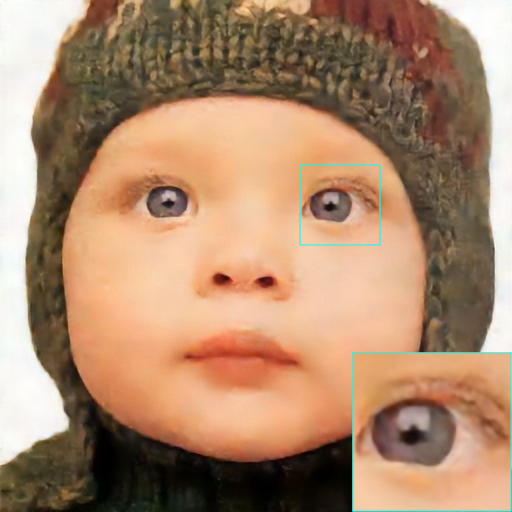
\includegraphics[width=\textwidth]{images/exp1.2/gaussian.png}
		\caption{Gaussian restored}
	\end{subfigure}
	\begin{subfigure}{0.24\textwidth}
		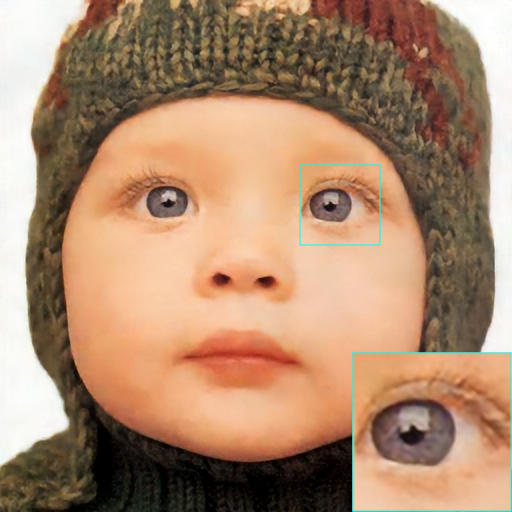
\includegraphics[width=\textwidth]{images/exp1.2/poisson.png}
		\caption{Poisson restored}
	\end{subfigure}
	\begin{subfigure}{0.24\textwidth}
		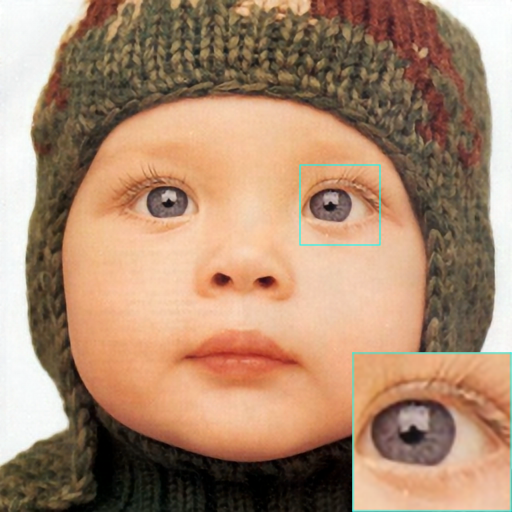
\includegraphics[width=\textwidth]{images/exp1.2/salt.png}
		\caption{S\&P restored}
	\end{subfigure}
	\begin{subfigure}{0.24\textwidth}
		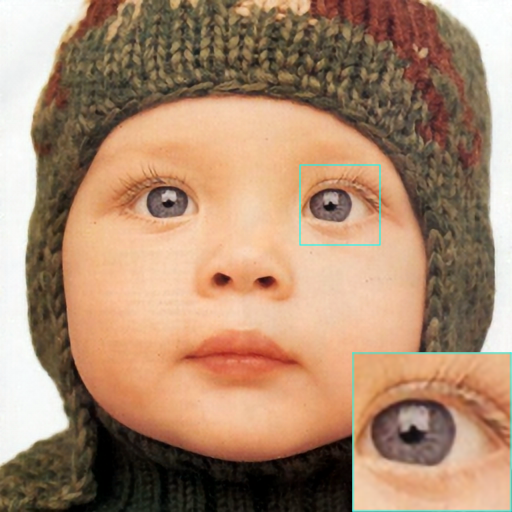
\includegraphics[width=\textwidth]{images/exp1.2/uniform.png}
		\caption{Uniform restored}
	\end{subfigure}
	\caption{Experiment 1.2: restoration using \gls{ircnn} $+$ \gls{fsrcnn}}
	\label{fig:exp1.2}
\end{figure}

In this case, \gls{ircnn} first removes the residual part, obtaining an approximation to the downscaled version of the \gls{hr} image. Once this is done, \gls{fsrcnn} super-resolves the denoised output in order to obtain the \gls{hr} image. 

Given these results, the next sets of experiments, which use both traditional and deep learning based methods, apply the algorithms following this logical order: the corresponding denoiser is applied (\gls{ircnn}, wavelet denoiser or median filter) followed by the \gls{sisr} algorithm (\gls{fsrcnn} or bicubic interpolation).


\newpage\subsection{Experiment 2.1}

In this experiment, we evaluate the results of replacing \gls{fsrcnn} by bicubic interpolation in the previous experiment. By doing this, we intend to analyze how a traditional method performs in comparison to a deep learning method when combined with \gls{ircnn}. The results of this experiment are exposed in Table \ref{tab:experiment21}.

\begin{table}[]
	\centering
	\begin{tabular}{|l|l|r|r|r|r|}
		\hline
		\rowcolor[HTML]{EFEFEF} 
		\multicolumn{1}{|c|}{\cellcolor[HTML]{EFEFEF}\textbf{Noise}} & \textbf{Parameters} & \multicolumn{1}{c|}{\cellcolor[HTML]{EFEFEF}\textbf{Set5 \gls{psnr}}} & \multicolumn{1}{c|}{\cellcolor[HTML]{EFEFEF}\textbf{Set5 \gls{ssim}}} & \multicolumn{1}{c|}{\cellcolor[HTML]{EFEFEF}\textbf{Set14 \gls{psnr} (dB)}} & \multicolumn{1}{c|}{\cellcolor[HTML]{EFEFEF}\textbf{Set14 \gls{ssim}}} \\ \hline
		\rowcolor[HTML]{FFFFFF} 
		\cellcolor[HTML]{EFEFEF} & $\mu=0, \sigma=0.05$ & 29.1069 & 0.9188 & 26.7379 & 0.8608 \\
		\rowcolor[HTML]{EFEFEF} 
		\cellcolor[HTML]{EFEFEF} & $\mu=0, \sigma=0.10$ & 27.3585 & 0.8963 & 25.4602 & 0.8206 \\
		\rowcolor[HTML]{FFFFFF} 
		\multirow{-3}{*}{\cellcolor[HTML]{EFEFEF}Gaussian} & $\mu=0, \sigma=0.15$ & 26.1240 & 0.8824 & 24.4524 & 0.7874 \\
		\rowcolor[HTML]{EFEFEF} 
		Poisson & $peak=2^8$ & 29.7801 & 0.9419 & 27.0475 & 0.8742 \\
		\rowcolor[HTML]{FFFFFF} 
		\cellcolor[HTML]{EFEFEF} & $r=0.05$ & 31.2225 & 0.9585 & 27.9022 & 0.8994 \\
		\rowcolor[HTML]{EFEFEF} 
		\cellcolor[HTML]{EFEFEF} & $r=0.10$ & 30.9084 & 0.9538 & 27.7169 & 0.8953 \\
		\rowcolor[HTML]{FFFFFF} 
		\cellcolor[HTML]{EFEFEF} & $r=0.15$ & 30.5699 & 0.9503 & 27.5133 & 0.8908 \\
		\rowcolor[HTML]{EFEFEF} 
		\multirow{-4}{*}{\cellcolor[HTML]{EFEFEF}Salt-and-pepper} & $r=0.20$ & 30.1156 & 0.9454 & 27.2382 & 0.8842 \\
		\rowcolor[HTML]{FFFFFF} 
		\cellcolor[HTML]{EFEFEF} & $r=0.05$ & 31.1893 & 0.9577 & 27.8885 & 0.8988 \\
		\rowcolor[HTML]{EFEFEF} 
		\cellcolor[HTML]{EFEFEF} & $r=0.10$ & 30.7560 & 0.9519 & 27.6282 & 0.8933 \\
		\rowcolor[HTML]{FFFFFF} 
		\cellcolor[HTML]{EFEFEF} & $r=0.15$ & 30.2349 & 0.9463 & 27.2898 & 0.8858 \\
		\rowcolor[HTML]{EFEFEF} 
		\multirow{-4}{*}{\cellcolor[HTML]{EFEFEF}Uniform} & $r=0.20$ & 29.5822 & 0.9393 & 26.8459 & 0.8753 \\
		\rowcolor[HTML]{FFFFFF} 
		\textbf{All} &  & \textbf{29.7457} & \textbf{0.9369} & \textbf{26.9767} & \textbf{0.8722}\\\hline
	\end{tabular}
	\caption{\gls{psnr} and \gls{ssim} results for the Experiment 2.1}
	\label{tab:experiment21}
\end{table}

In the table, we can see that, in average, the overall \gls{psnr} and \gls{ssim} results are $0.5732dB$ and $0.0028$ units lower than the results of Experiment 1.2, respectively. However, if we take a look at the \gls{ssim} results on the five images of Set5, we see a slight improvement when we choose bicubic interpolation over \gls{fsrcnn}.

In Figure \ref{fig:exp2.1}, we present the results of applying \gls{ircnn} $+$ bicubic interpolation to the images of Figure \ref{fig:exp0}. In this case, we can see that the bicubic interpolation provides good results as well, however it cannot conserve the image edges as well as \gls{fsrcnn} does when super-resolving the \gls{lr} images.

\begin{figure}
	\centering
	\begin{subfigure}{0.24\textwidth}
		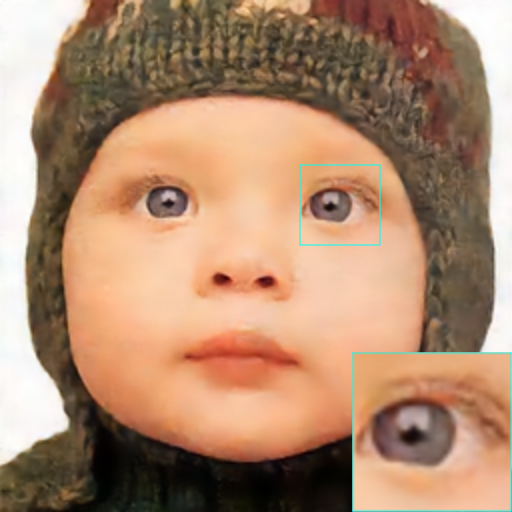
\includegraphics[width=\textwidth]{images/exp2.1/gaussian.png}
		\caption{Gaussian restored}
	\end{subfigure}
	\begin{subfigure}{0.24\textwidth}
		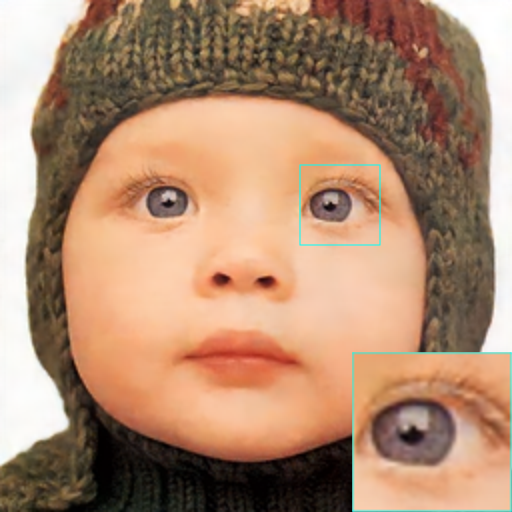
\includegraphics[width=\textwidth]{images/exp2.1/poisson.png}
		\caption{Poisson restored}
	\end{subfigure}
	\begin{subfigure}{0.24\textwidth}
		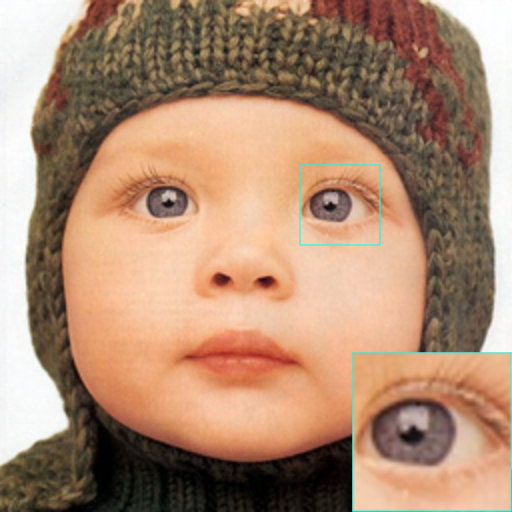
\includegraphics[width=\textwidth]{images/exp2.1/salt.png}
		\caption{S\&P restored}
	\end{subfigure}
	\begin{subfigure}{0.24\textwidth}
		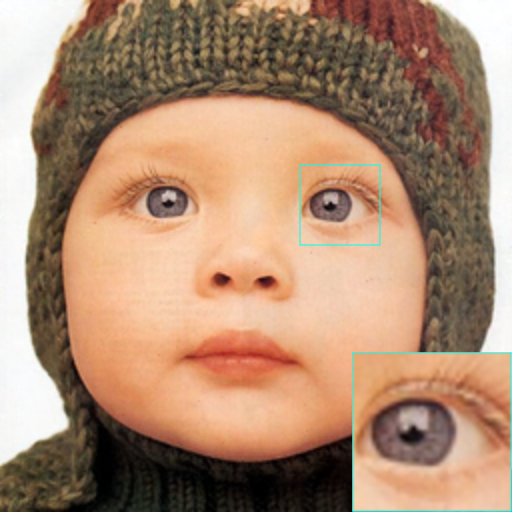
\includegraphics[width=\textwidth]{images/exp2.1/uniform.png}
		\caption{Uniform restored}
	\end{subfigure}
	\caption{Experiment 2.1: restoration using \gls{ircnn} $+$ bicubic interpolation}
	\label{fig:exp2.1}
\end{figure}

These results show that even though in average \gls{fsrcnn} performs better, there might be some cases in which the bicubic interpolation approximates better the original \gls{hr} image.

However, the performance of the \gls{sisr} algorithms is being compared using the output of \gls{ircnn} as an input, which is the result of convolving the noisy \gls{lr} image with the corresponding \gls{ircnn} filters. Hence, even though the \gls{ssim} results for Set5 show better performance for bicubic interpolation, we show in Table \ref{tab:experiment} that \gls{fsrcnn} overperforms bicubic interpolation if we use the downscaled images without noise as the input of both algorithms.

\begin{table}[]
	\centering
	\begin{tabular}{|l|r|r|r|r|}
		\hline
		\rowcolor[HTML]{EFEFEF}
		\multicolumn{1}{|c}{\cellcolor[HTML]{EFEFEF}\textbf{Method}} &
		\multicolumn{1}{c|}{\cellcolor[HTML]{EFEFEF}\textbf{Set5 \gls{psnr} (dB)}} & \multicolumn{1}{c|}{\cellcolor[HTML]{EFEFEF}\textbf{Set5 \gls{ssim}}} & \multicolumn{1}{c|}{\cellcolor[HTML]{EFEFEF}\textbf{Set14 \gls{psnr} (dB)}} & \multicolumn{1}{c|}{\cellcolor[HTML]{EFEFEF}\textbf{Set14 \gls{ssim}}} \\ \hline
		\rowcolor[HTML]{FFFFFF} 
		\gls{fsrcnn} & 33.9226 & 0.9733 & 29.8034 & 0.9304\\
		\rowcolor[HTML]{EFEFEF} 
		Bicubic Interpolation & 32.2347 & 0.9677 & 28.6030 & 0.9115\\\hline
		\textbf{\gls{fsrcnn} - Bicubic} & \textbf{+1.6879} & \textbf{+0.0056} & \textbf{+1.2004} & \textbf{+0.0189}\\\hline
	\end{tabular}
	\caption{\gls{psnr} and \gls{ssim} results for \gls{fsrcnn} vs Bicubic Interpolation on the downscaled images of Set5 and Set14.}
	\label{tab:experiment}
\end{table}

\newpage\subsection{Experiment 2.2}
In this experiment, we evaluate the results of applying wavelet denoiser $+$ \gls{fsrcnn}. In this case, instead of substituting the super-resolution algorithm, we keep \gls{fsrcnn} for the \gls{sisr} task and replace \gls{ircnn} by a wavelet denoiser. The results of this experiment are exposed in Table \ref{tab:experiment22}.

\begin{table}[]
	\centering
	\begin{tabular}{|l|l|r|r|r|r|}
		\hline
		\rowcolor[HTML]{EFEFEF} 
		\multicolumn{1}{|c|}{\cellcolor[HTML]{EFEFEF}\textbf{Noise}} & \textbf{Parameters} & \multicolumn{1}{c|}{\cellcolor[HTML]{EFEFEF}\textbf{Set5 \gls{psnr} (dB)}} & \multicolumn{1}{c|}{\cellcolor[HTML]{EFEFEF}\textbf{Set5 \gls{ssim}}} & \multicolumn{1}{c|}{\cellcolor[HTML]{EFEFEF}\textbf{Set14 \gls{psnr} (dB)}} & \multicolumn{1}{c|}{\cellcolor[HTML]{EFEFEF}\textbf{Set14 \gls{ssim}}} \\ \hline
		\rowcolor[HTML]{FFFFFF} 
		\cellcolor[HTML]{EFEFEF} & $\mu=0, \sigma=0.05$ & 27.8830 & 0.9132 & 25.8943 & 0.8294 \\
		\rowcolor[HTML]{EFEFEF} 
		\cellcolor[HTML]{EFEFEF} & $\mu=0, \sigma=0.10$ & 25.0741 & 0.8574 & 23.6262 & 0.7520 \\
		\rowcolor[HTML]{FFFFFF} 
		\multirow{-3}{*}{\cellcolor[HTML]{EFEFEF}Gaussian} & $\mu=0, \sigma=0.15$ & 23.2414 & 0.8060 & 22.2485 & 0.7009 \\
		\rowcolor[HTML]{EFEFEF} 
		Poisson & $peak=2^8$ & 28.6318 & 0.9219 & 26.4398 & 0.8493 \\
		\rowcolor[HTML]{FFFFFF} 
		\cellcolor[HTML]{EFEFEF} & $r=0.05$ & 19.7492 & 0.6890 & 19.8054 & 0.6197 \\
		\rowcolor[HTML]{EFEFEF} 
		\cellcolor[HTML]{EFEFEF} & $r=0.10$ & 19.3873 & 0.6486 & 19.4879 & 0.5753 \\
		\rowcolor[HTML]{FFFFFF} 
		\cellcolor[HTML]{EFEFEF} & $r=0.15$ & 19.2579 & 0.6496 & 19.3416 & 0.5734 \\
		\rowcolor[HTML]{EFEFEF} 
		\multirow{-4}{*}{\cellcolor[HTML]{EFEFEF}Salt-and-pepper} & $r=0.20$ & 18.8251 & 0.6435 & 18.9623 & 0.5686 \\
		\rowcolor[HTML]{FFFFFF} 
		\cellcolor[HTML]{EFEFEF} & $r=0.05$ & 22.0364 & 0.7589 & 21.8637 & 0.7057 \\
		\rowcolor[HTML]{EFEFEF} 
		\cellcolor[HTML]{EFEFEF} & $r=0.10$ & 20.8710 & 0.7059 & 20.7881 & 0.6402 \\
		\rowcolor[HTML]{FFFFFF} 
		\cellcolor[HTML]{EFEFEF} & $r=0.15$ & 20.1205 & 0.6836 & 20.1378 & 0.6124 \\
		\rowcolor[HTML]{EFEFEF} 
		\multirow{-4}{*}{\cellcolor[HTML]{EFEFEF}Uniform} & $r=0.20$ & 19.3803 & 0.6659 & 19.5532 & 0.5959 \\
		\rowcolor[HTML]{FFFFFF} 
		\textbf{All} &  & \textbf{22.0382} & \textbf{0.7453} & \textbf{21.5124} & \textbf{0.6686}\\\hline
	\end{tabular}
	\caption{\gls{psnr} and \gls{ssim} results for the Experiment 2.2}
	\label{tab:experiment22}
\end{table}

In the table, we can observe that the \gls{psnr} and \gls{ssim} results are worse than the ones obtained in the experiments using \gls{ircnn} as a denoiser. These results can also be observed in Figure \ref{fig:exp2.2}, in which wavelet denoiser $+$ \gls{fsrcnn} are applied on the images of Figure \ref{fig:exp0}.

\begin{figure}
	\centering
	\begin{subfigure}{0.24\textwidth}
		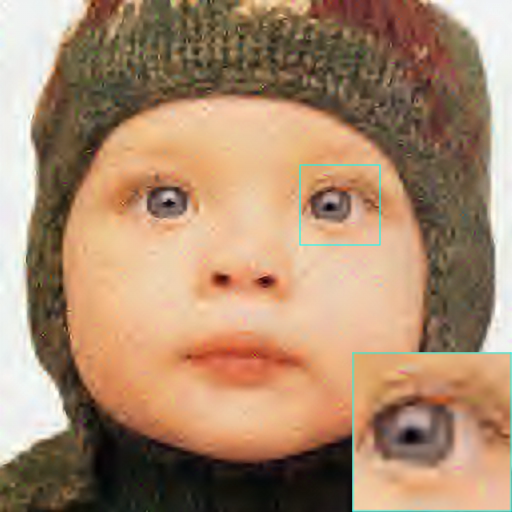
\includegraphics[width=\textwidth]{images/exp2.2/gaussian.png}
		\caption{Gaussian restored}
	\end{subfigure}
	\begin{subfigure}{0.24\textwidth}
		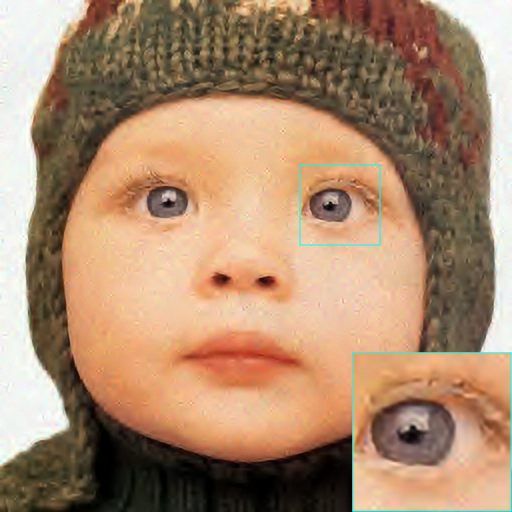
\includegraphics[width=\textwidth]{images/exp2.2/poisson.png}
		\caption{Poisson restored}
	\end{subfigure}
	\begin{subfigure}{0.24\textwidth}
		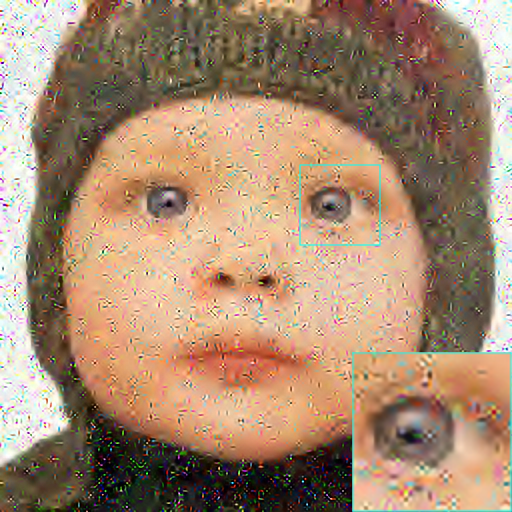
\includegraphics[width=\textwidth]{images/exp2.2/salt.png}
		\caption{S\&P restored}
	\end{subfigure}
	\begin{subfigure}{0.24\textwidth}
		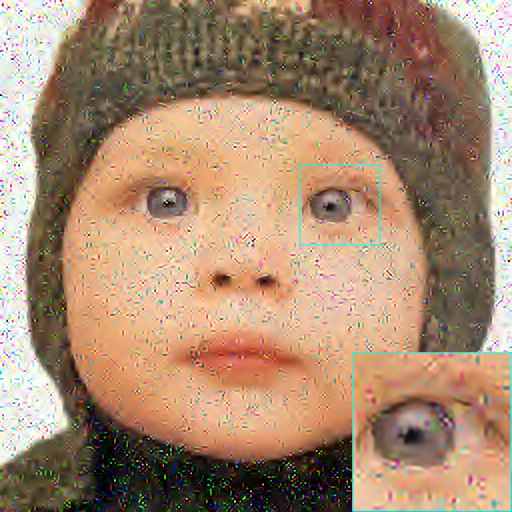
\includegraphics[width=\textwidth]{images/exp2.2/uniform.png}
		\caption{Uniform restored}
	\end{subfigure}
	\caption{Experiment 2.2: restoration using wavelet denoiser $+$ \gls{fsrcnn}}
	\label{fig:exp2.2}
\end{figure}

In the first instance, the wavelet denoiser is able to effectively reduce the noise for those types that are additive or signal dependent, i.e., the Gaussian noise and the Poisson noise. However, the quality of the results is not as high as in the \gls{ircnn} results. 

On the other hand, if we take a look at the results of this combination on the images degraded by salt-and-pepper noise and uniform noise, we can observe that the wavelet algorithm cannot properly remove the noise, and therefore the final images present low-quality.

\newpage\subsection{Experiment 2.3}
In this experiment, we replace the wavelet denoiser of the previous experiment by a median filter. Therefore, we evaluate the results of applying a median filter + \gls{fsrcnn} on our set of \gls{lr} images. The metrics results of this experiment are presented in Table \ref{tab:experiment23}.

\begin{table}[]
	\centering
	\begin{tabular}{|l|l|r|r|r|r|}
		\hline
		\rowcolor[HTML]{EFEFEF} 
		\multicolumn{1}{|c|}{\cellcolor[HTML]{EFEFEF}\textbf{Noise}} & \textbf{Parameters} & \multicolumn{1}{c|}{\cellcolor[HTML]{EFEFEF}\textbf{Set5 \gls{psnr} (dB)}} & \multicolumn{1}{c|}{\cellcolor[HTML]{EFEFEF}\textbf{Set5 \gls{ssim}}} & \multicolumn{1}{c|}{\cellcolor[HTML]{EFEFEF}\textbf{Set14 \gls{psnr} (dB)}} & \multicolumn{1}{c|}{\cellcolor[HTML]{EFEFEF}\textbf{Set14 \gls{ssim}}} \\ \hline
		\rowcolor[HTML]{FFFFFF} 
		\cellcolor[HTML]{EFEFEF} & $\mu=0, \sigma=0.05$ & 25.9872 & 0.8739 & 23.9859 & 0.7578 \\
		\rowcolor[HTML]{EFEFEF} 
		\cellcolor[HTML]{EFEFEF} & $\mu=0, \sigma=0.10$ & 23.9557 & 0.8044 & 22.5017 & 0.6852 \\
		\rowcolor[HTML]{FFFFFF} 
		\multirow{-3}{*}{\cellcolor[HTML]{EFEFEF}Gaussian} & $\mu=0, \sigma=0.15$ & 22.0852 & 0.7334 & 20.9973 & 0.6142 \\
		\rowcolor[HTML]{EFEFEF} 
		Poisson & $peak=2^8$ & 26.2772 & 0.8925 & 24.1578 & 0.7690 \\
		\rowcolor[HTML]{FFFFFF} 
		\cellcolor[HTML]{EFEFEF} & $r=0.05$ & 26.8715 & 0.9165 & 24.5762 & 0.7983 \\
		\rowcolor[HTML]{EFEFEF} 
		\cellcolor[HTML]{EFEFEF} & $r=0.10$ & 26.0928 & 0.9069 & 24.0433 & 0.7888 \\
		\rowcolor[HTML]{FFFFFF} 
		\cellcolor[HTML]{EFEFEF} & $r=0.15$ & 25.1191 & 0.8942 & 23.3845 & 0.7751 \\
		\rowcolor[HTML]{EFEFEF} 
		\multirow{-4}{*}{\cellcolor[HTML]{EFEFEF}Salt-and-pepper} & $r=0.20$ & 23.8783 & 0.8750 & 22.5070 & 0.7551 \\
		\rowcolor[HTML]{FFFFFF} 
		\cellcolor[HTML]{EFEFEF} & $r=0.05$ & 26.9496 & 0.9171 & 24.6094 & 0.7979 \\
		\rowcolor[HTML]{EFEFEF} 
		\cellcolor[HTML]{EFEFEF} & $r=0.10$ & 26.2939 & 0.9076 & 24.2091 & 0.7878 \\
		\rowcolor[HTML]{FFFFFF} 
		\cellcolor[HTML]{EFEFEF} & $r=0.15$ & 25.5000 & 0.8921 & 23.6985 & 0.7726 \\
		\rowcolor[HTML]{EFEFEF} 
		\multirow{-4}{*}{\cellcolor[HTML]{EFEFEF}Uniform} & $r=0.20$ & 24.4354 & 0.8651 & 23.0633 & 0.7503 \\
		\rowcolor[HTML]{FFFFFF} 
		\textbf{All} &  & \textbf{25.2872} & \textbf{0.8732} & \textbf{23.4778} & \textbf{0.7543}\\\hline
	\end{tabular}
	\caption{\gls{psnr} and \gls{ssim} results for the Experiment 2.3}
	\label{tab:experiment23}
\end{table}

In the table, we can see that the average \gls{psnr} and \gls{ssim} results improve when we replace the wavelet denoiser by a median filter. However, even though the overall results and the results obtained on the images degraded with salt-and-pepper and uniform noise are better compared to the previous experiment, the wavelet denoiser overperforms the median filter on the images that were degraded with Gaussian and Poisson noise.

\begin{figure}
	\centering
	\begin{subfigure}{0.24\textwidth}
		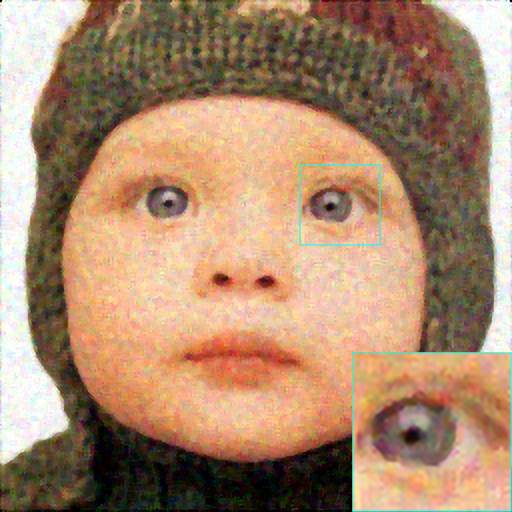
\includegraphics[width=\textwidth]{images/exp2.3/gaussian.png}
		\caption{Gaussian restored}
	\end{subfigure}
	\begin{subfigure}{0.24\textwidth}
		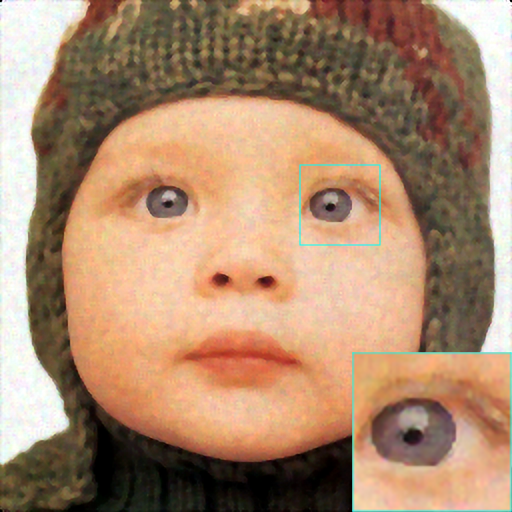
\includegraphics[width=\textwidth]{images/exp2.3/poisson.png}
		\caption{Poisson restored}
	\end{subfigure}
	\begin{subfigure}{0.24\textwidth}
		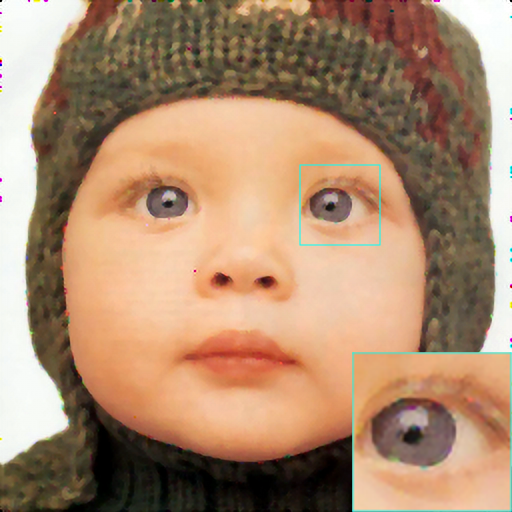
\includegraphics[width=\textwidth]{images/exp2.3/salt.png}
		\caption{S\&P restored}
	\end{subfigure}
	\begin{subfigure}{0.24\textwidth}
		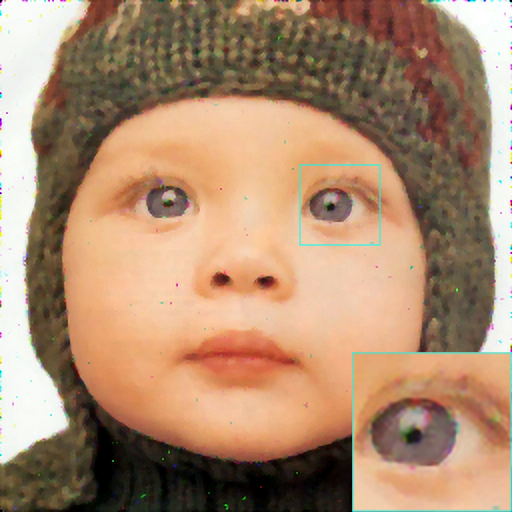
\includegraphics[width=\textwidth]{images/exp2.3/uniform.png}
		\caption{Uniform restored}
	\end{subfigure}
	\caption{Experiment 2.3: restoration using median filter $+$ \gls{fsrcnn}}
	\label{fig:exp2.3}
\end{figure}

This can also be observed in Figure \ref{fig:exp2.3}, in which we present the results of applying median filter $+$ \gls{fsrcnn} to the images of Figure \ref{fig:exp0}. The images with Gaussian and Poisson noise still present a considerable amount of noise after the restoration. On the other hand, the images degraded with salt-and-pepper and uniform noise present a much lower amount of noise after applying the median filter. 

In any case, the performance obtained in Experiment 1.2. cannot be reached by using any of these traditional filters.

\newpage\subsection{Experiment 3.1}
In this experiment we use a traditional approach for both tasks: a wavelet denoiser is used for image denoising and bicubic interpolation is used for super-resolution. Table \ref{tab:experiment31} shows the results of the quality metrics for this experiment.

\begin{table}[]
	\centering
	\begin{tabular}{|l|l|r|r|r|r|}
		\hline
		\rowcolor[HTML]{EFEFEF} 
		\multicolumn{1}{|c|}{\cellcolor[HTML]{EFEFEF}\textbf{Noise}} & \textbf{Parameters} & \multicolumn{1}{c|}{\cellcolor[HTML]{EFEFEF}\textbf{Set5 \gls{psnr} (dB)}} & \multicolumn{1}{c|}{\cellcolor[HTML]{EFEFEF}\textbf{Set5 \gls{ssim}}} & \multicolumn{1}{c|}{\cellcolor[HTML]{EFEFEF}\textbf{Set14 \gls{psnr} (dB)}} & \multicolumn{1}{c|}{\cellcolor[HTML]{EFEFEF}\textbf{Set14 \gls{ssim}}} \\ \hline
		\rowcolor[HTML]{FFFFFF} 
		\cellcolor[HTML]{EFEFEF} & $\mu=0, \sigma=0.05$ & 27.8760 & 0.9116 & 25.8165 & 0.8244 \\
		\rowcolor[HTML]{EFEFEF} 
		\cellcolor[HTML]{EFEFEF} & $\mu=0, \sigma=0.10$ & 25.2040 & 0.8553 & 23.7390 & 0.7520 \\
		\rowcolor[HTML]{FFFFFF} 
		\multirow{-3}{*}{\cellcolor[HTML]{EFEFEF}Gaussian} & $\mu=0, \sigma=0.15$ & 23.3125 & 0.8046 & 22.3406 & 0.7016 \\
		\rowcolor[HTML]{EFEFEF} 
		Poisson & $peak=2^8$ & 28.7267 & 0.9298 & 26.3338 & 0.8453 \\
		\rowcolor[HTML]{FFFFFF} 
		\cellcolor[HTML]{EFEFEF} & $r=0.05$ & 20.8489 & 0.7180 & 20.8049 & 0.6445 \\
		\rowcolor[HTML]{EFEFEF} 
		\cellcolor[HTML]{EFEFEF} & $r=0.10$ & 20.0257 & 0.6657 & 20.0924 & 0.5918 \\
		\rowcolor[HTML]{FFFFFF} 
		\cellcolor[HTML]{EFEFEF} & $r=0.15$ & 19.5516 & 0.6569 & 19.6361 & 0.5817 \\
		\rowcolor[HTML]{EFEFEF} 
		\multirow{-4}{*}{\cellcolor[HTML]{EFEFEF}Salt-and-pepper} & $r=0.20$ & 18.9040 & 0.6454 & 19.0571 & 0.5714 \\
		\rowcolor[HTML]{FFFFFF} 
		\cellcolor[HTML]{EFEFEF} & $r=0.05$ & 22.9494 & 0.7780 & 22.6777 & 0.7204 \\
		\rowcolor[HTML]{EFEFEF} 
		\cellcolor[HTML]{EFEFEF} & $r=0.10$ & 21.4818 & 0.7196 & 21.3892 & 0.6547 \\
		\rowcolor[HTML]{FFFFFF} 
		\cellcolor[HTML]{EFEFEF} & $r=0.15$ & 20.4685 & 0.6920 & 20.5239 & 0.6233 \\
		\rowcolor[HTML]{EFEFEF} 
		\multirow{-4}{*}{\cellcolor[HTML]{EFEFEF}Uniform} & $r=0.20$ & 19.5550 & 0.6708 & 19.7700 & 0.6028 \\
		\rowcolor[HTML]{FFFFFF} 
		\textbf{All} &  & \textbf{22.4087} & \textbf{0.7540} & \textbf{21.8485} & \textbf{0.6762}\\\hline
	\end{tabular}
	\caption{\gls{psnr} and \gls{ssim} results for the Experiment 3.1}
	\label{tab:experiment31}
\end{table}

In the table, we can see that the \gls{psnr} and \gls{ssim} results are very similar to the ones of Experiment 2.2. In this case, replacing \gls{fsrcnn} by bicubic interpolation does not bring any improvement due to the fact that the super-resolution task is being performed using images which have been denoised with low quality outputs.

Figure \ref{fig:exp3.1} shows the results of applying a wavelet denoiser $+$ bicubic interpolation to the images of Figure \ref{fig:exp0}. In Figure \ref{fig:exp3.1}, we can see the same effect as in Experiment 2.2: even though the wavelet denoiser is able to remove Gaussian and Poisson noise, the obtained quality is not high enough, and the denoising results are not acceptable for salt-and-pepper and uniform noise.

\begin{figure}
	\centering
	\begin{subfigure}{0.24\textwidth}
		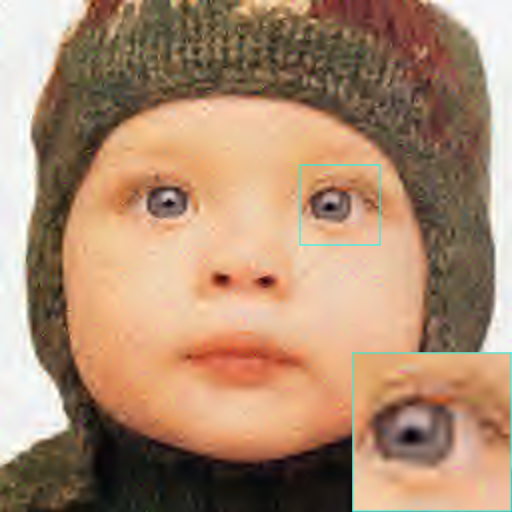
\includegraphics[width=\textwidth]{images/exp3.1/gaussian.png}
		\caption{Gaussian restored}
	\end{subfigure}
	\begin{subfigure}{0.24\textwidth}
		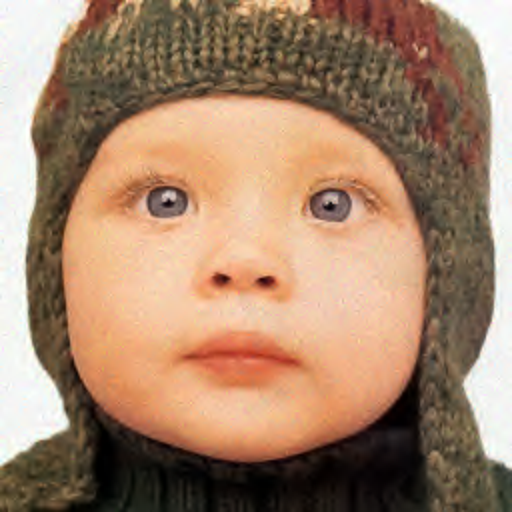
\includegraphics[width=\textwidth]{images/exp3.1/poisson.png}
		\caption{Poisson restored}
	\end{subfigure}
	\begin{subfigure}{0.24\textwidth}
		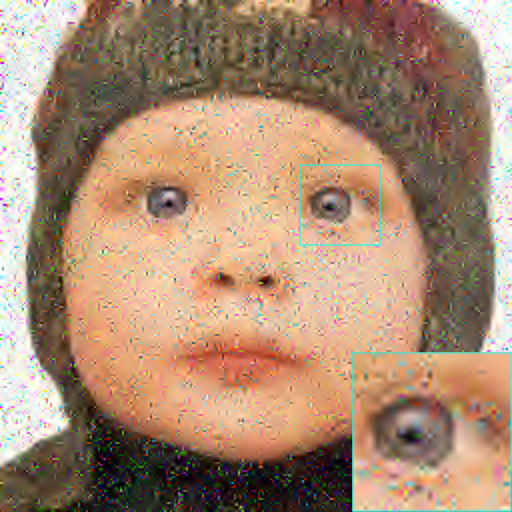
\includegraphics[width=\textwidth]{images/exp3.1/salt.png}
		\caption{S\&P restored}
	\end{subfigure}
	\begin{subfigure}{0.24\textwidth}
		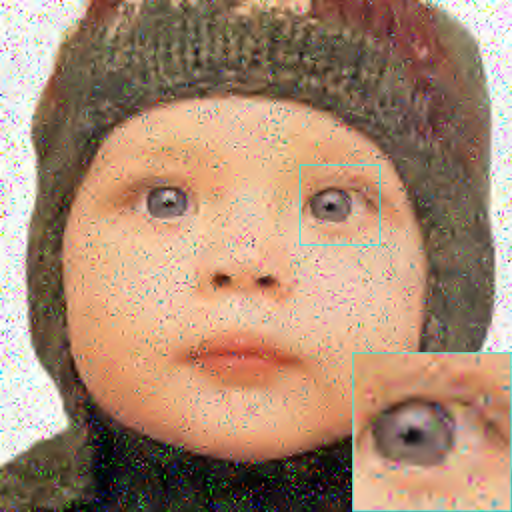
\includegraphics[width=\textwidth]{images/exp3.1/uniform.png}
		\caption{Uniform restored}
	\end{subfigure}
	\caption{Experiment 3.1: restoration using wavelet denoiser $+$ bicubic interpolation}
	\label{fig:exp3.1}
\end{figure}

Therefore, although \gls{fsrcnn} is able to outperform bicubic interpolation in most of the cases, in this experiment its inputs are degraded by the applied noise, affecting the quality of the super-resolution process.

\newpage\subsection{Experiment 3.2}
In this experiment we evaluate the performance of applying median filter $+$ bicubic interpolation on our set of degraded images. The results of this experiment are exposed in Table \ref{tab:experiment32}.

\begin{table}[]
	\centering
	\begin{tabular}{|l|l|r|r|r|r|}
		\hline
		\rowcolor[HTML]{EFEFEF} 
		\multicolumn{1}{|c|}{\cellcolor[HTML]{EFEFEF}\textbf{Noise}} & \textbf{Parameters} & \multicolumn{1}{c|}{\cellcolor[HTML]{EFEFEF}\textbf{Set5 \gls{psnr} (dB)}} & \multicolumn{1}{c|}{\cellcolor[HTML]{EFEFEF}\textbf{Set5 \gls{ssim}}} & \multicolumn{1}{c|}{\cellcolor[HTML]{EFEFEF}\textbf{Set14 \gls{psnr} (dB)}} & \multicolumn{1}{c|}{\cellcolor[HTML]{EFEFEF}\textbf{Set14 \gls{ssim}}} \\ \hline
		\rowcolor[HTML]{FFFFFF} 
		\cellcolor[HTML]{EFEFEF} & $\mu=0, \sigma=0.05$ & 26.2755 & 0.8812 & 24.2264 & 0.7663 \\
		\rowcolor[HTML]{EFEFEF} 
		\cellcolor[HTML]{EFEFEF} & $\mu=0, \sigma=0.10$ & 24.2735 & 0.8134 & 22.8012 & 0.6979 \\
		\rowcolor[HTML]{FFFFFF} 
		\multirow{-3}{*}{\cellcolor[HTML]{EFEFEF}Gaussian} & $\mu=0, \sigma=0.15$ & 22.4366 & 0.7452 & 21.3403 & 0.6299 \\
		\rowcolor[HTML]{EFEFEF} 
		Poisson & $peak=2^8$ & 26.6459 & 0.9059 & 24.4262 & 0.7795 \\
		\rowcolor[HTML]{FFFFFF} 
		\cellcolor[HTML]{EFEFEF} & $r=0.05$ & 27.1121 & 0.9209 & 24.7449 & 0.8034 \\
		\rowcolor[HTML]{EFEFEF} 
		\cellcolor[HTML]{EFEFEF} & $r=0.10$ & 26.3782 & 0.9123 & 24.2646 & 0.7950 \\
		\rowcolor[HTML]{FFFFFF} 
		\cellcolor[HTML]{EFEFEF} & $r=0.15$ & 25.4810 & 0.9009 & 23.6647 & 0.7829 \\
		\rowcolor[HTML]{EFEFEF} 
		\multirow{-4}{*}{\cellcolor[HTML]{EFEFEF}Salt-and-pepper} & $r=0.20$ & 24.3109 & 0.8836 & 22.8559 & 0.7650 \\
		\rowcolor[HTML]{FFFFFF} 
		\cellcolor[HTML]{EFEFEF} & $r=0.05$ & 27.1583 & 0.9208 & 24.7666 & 0.8026 \\
		\rowcolor[HTML]{EFEFEF} 
		\cellcolor[HTML]{EFEFEF} & $r=0.10$ & 26.5295 & 0.9116 & 24.3931 & 0.7933 \\
		\rowcolor[HTML]{FFFFFF} 
		\cellcolor[HTML]{EFEFEF} & $r=0.15$ & 25.7746 & 0.8967 & 23.9241 & 0.7793 \\
		\rowcolor[HTML]{EFEFEF} 
		\multirow{-4}{*}{\cellcolor[HTML]{EFEFEF}Uniform} & $r=0.20$ & 24.7671 & 0.8715 & 23.3377 & 0.7590 \\
		\rowcolor[HTML]{FFFFFF} 
		\textbf{All} &  & \textbf{25.5953} & \textbf{0.8803} & \textbf{23.7288} & \textbf{0.7628}\\\hline
	\end{tabular}
	\caption{\gls{psnr} and \gls{ssim} results for the Experiment 3.2}
	\label{tab:experiment32}
\end{table}

In the table, we can observe that the obtained quality results are similar to the ones of Experiment 2.3. As in the previous experiment, the denoiser is not able to provide high denoising quality and therefore the super-resolution step is performed using noisy images.



\begin{figure}
	\centering
	\begin{subfigure}{0.24\textwidth}
		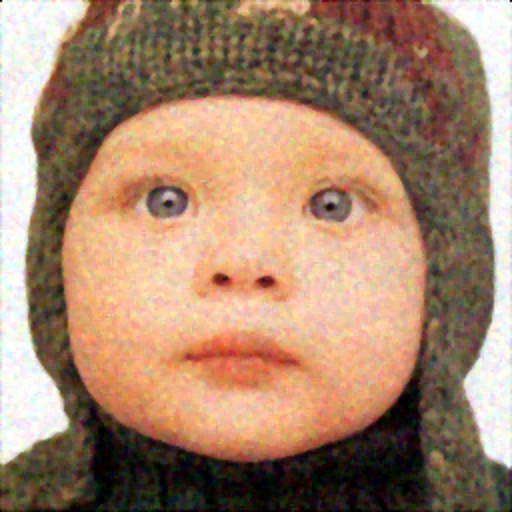
\includegraphics[width=\textwidth]{images/exp3.2/gaussian.png}
		\caption{Gaussian restored}
	\end{subfigure}
	\begin{subfigure}{0.24\textwidth}
		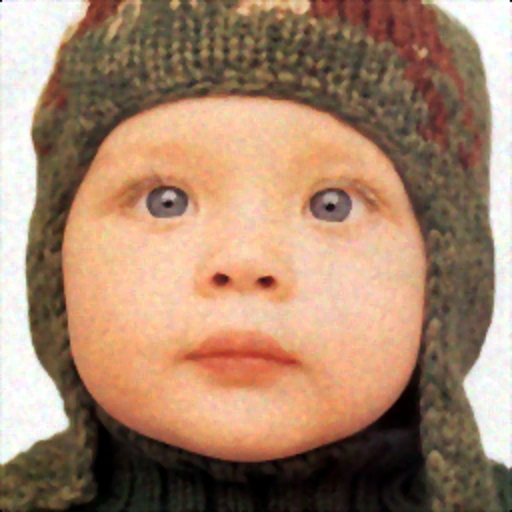
\includegraphics[width=\textwidth]{images/exp3.2/poisson.png}
		\caption{Poisson restored}
	\end{subfigure}
	\begin{subfigure}{0.24\textwidth}
		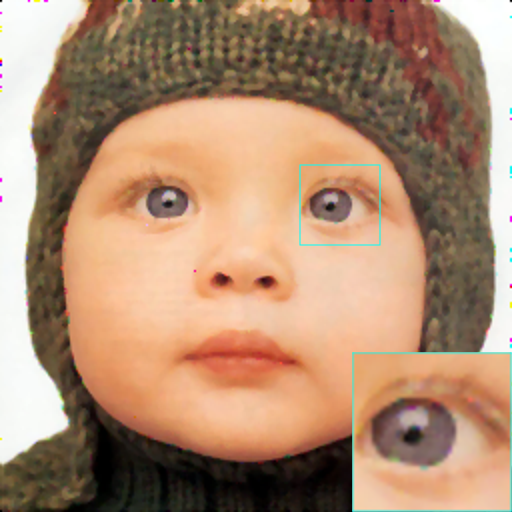
\includegraphics[width=\textwidth]{images/exp3.2/salt.png}
		\caption{S\&P restored}
	\end{subfigure}
	\begin{subfigure}{0.24\textwidth}
		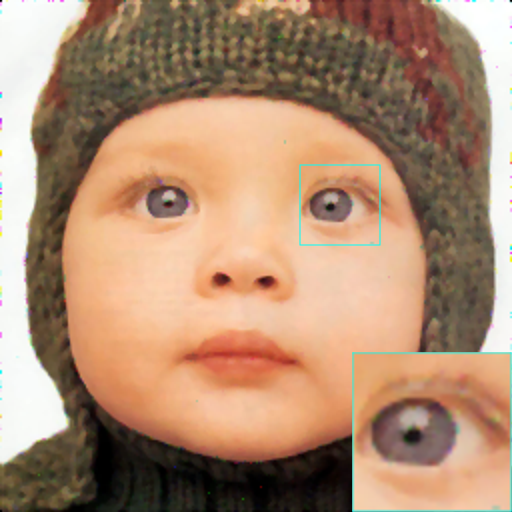
\includegraphics[width=\textwidth]{images/exp3.2/uniform.png}
		\caption{Uniform restored}
	\end{subfigure}
	\caption{Experiment 3.2: restoration using median filter $+$ bicubic interpolation}
	\label{fig:exp3.2}
\end{figure}

In Figure \ref{fig:exp3.2} we present the results of applying median filter $+$ bicubic interpolation on the images of Figure \ref{fig:exp0}. Once more, we can see results that are similar to the Experiment 2.3: the images degraded with Gaussian and Poisson noise still have a considerable amount of noise, whereas the noise in the images that presented salt-and-pepper and uniform noise is lower.

\subsection{Results summary}
In this section we summarize the results of all the experiments carried out for this study. Table \ref{tab:expsum} presents a summary of the \gls{psnr} and \gls{ssim} results for each of them.

First of all, we can see that both approaches that use a pure deep learning solution for the \gls{sisr} and denoising tasks present different results. Experiment 1.1 shows low restoration quality results because \gls{fsrcnn} mixes up the information contained in the pixels of the image with those that have lost information due to the applied noise. On the other hand, Experiment 1.2 presents much better results obtained by simply swapping the order in which the neural networks are applied.

In the rest of experiments, we compared the performance obtained when we replaced the \glspl{cnn} by traditional methods for the \gls{sisr} and denoising tasks. The results show that when we replace \gls{ircnn} by a wavelet denoiser or a median filter, the restoration quality decreases.

Furthermore, we have also observed that the results for the \gls{sisr} task are directly impacted by the performance of the denoising step. In fact, we can see in Table \ref{tab:expsum} that \gls{fsrcnn} is not able to overperform bicubic interpolation when we use traditional methods for the denoising.

The best restoration quality results are achieved by using the deep learning methods as long as the denoising step is performed before \gls{sisr}.


\begin{table}[]
	\centering
	\begin{tabular}{|l|l|r|r|}
		\hline
		\rowcolor[HTML]{EFEFEF} 
		\multicolumn{1}{|c|}{\cellcolor[HTML]{EFEFEF}\textbf{Experiment}} &
		\multicolumn{1}{c|}{\cellcolor[HTML]{EFEFEF}\textbf{Solution}} & \multicolumn{1}{c|}{\cellcolor[HTML]{EFEFEF}\textbf{\gls{psnr} (dB)}} & \multicolumn{1}{c|}{\cellcolor[HTML]{EFEFEF}\textbf{\gls{ssim}}} \\ \hline
		\rowcolor[HTML]{FFFFFF} 
		\cellcolor[HTML]{EFEFEF} Experiment 1.1 & \gls{fsrcnn} $+$ \gls{ircnn} & 20.2899 & 0.6399 \\
		\rowcolor[HTML]{EFEFEF} 
		\cellcolor[HTML]{EFEFEF} \textbf{Experiment 1.2} & \textbf{\gls{ircnn}} $+$ \textbf{\gls{fsrcnn}} & \textbf{28.9344} & \textbf{0.9073} \\
		\rowcolor[HTML]{FFFFFF} 
		\cellcolor[HTML]{EFEFEF} Experiment 2.1 & \gls{ircnn} $+$ Bicubic & 28.3612 & 0.9046\\
		\rowcolor[HTML]{EFEFEF} 
		\cellcolor[HTML]{EFEFEF} Experiment 2.2 & Wavelet $+$ \gls{fsrcnn} & 21.7753 & 0.7070 \\ 
		\rowcolor[HTML]{FFFFFF} 
		\cellcolor[HTML]{EFEFEF} Experiment 2.3 & Median $+$ \gls{fsrcnn} & 24.3825 & 0.8138 \\
		\rowcolor[HTML]{EFEFEF} 
		\cellcolor[HTML]{EFEFEF} Experiment 3.1 & Wavelet $+$ Bicubic & 22.1286 & 0.7151 \\ 
		\rowcolor[HTML]{FFFFFF} 
		\cellcolor[HTML]{EFEFEF} Experiment 3.2 & Median $+$ Bicubic & 24.6621 & 0.8216 \\
		\hline
	\end{tabular}
	\caption{\gls{psnr} and \gls{ssim} results on Set5 and Set14}
	\label{tab:expsum}
\end{table}

	% !TeX spellcheck = en_US
\section{Conclusions and further developments} \label{sec:conclusions}

\gls{sisr} and image denoising are two important low-level computer vision tasks with multiple applications. In the last few decades, \glspl{cnn} have shown promising results while performing such kinds of restoration tasks, receiving increasing attention from researches.

In this study, we have analyzed the results of the combined application of two well known \glspl{cnn} for \gls{sisr} and image denoising: \gls{fsrcnn} and \gls{ircnn}, respectively.
Our results show that the order in which these algorithms are applied has a direct effect in their combined performance: if the \gls{sisr} algorithm is applied first, those pixels affected by the image noise will be convolved with the good information, producing low quality restoration results. Instead, if the denoiser is applied first, the \gls{sisr} will manage to super-resolve the \gls{lr} image.

For this analysis, both \gls{cnn} have been trained using the same images from BSD200 \cite{BSDS}, General100 \cite{FSRCNN} and T91 \cite{T91} datasets. A Keras \cite{KERAS} is also provided with this study.

Furthermore, we have carried out a set of experiments comparing the performance of these deep learning methods to traditional algorithms for the \gls{sisr} and denoising tasks. In all the cases, the combination of \gls{ircnn} and \gls{fsrcnn} shows better performance than when bicubic interpolation is used for \gls{sisr} and wavelet denoising or median filtering is applied for denoising.

Although the results of this study show that the deep learning approach using \gls{ircnn} + \gls{fsrcnn} overperforms the selected traditional methods, there remain several open questions for future research works.

First of all, most of the research studies simulate the \gls{lr} images by modeling the degradation with algorithms like bicubic or Lanczos interpolation and Gaussian noise, whereas in real scenarios the \gls{lr} images may present a different distribution, and therefore the learned mappings might not be useful for these cases.

Furthermore, a more extensive comparison with other traditional methods for \gls{sisr} and image denoising could be addressed, including algorithms such as total variation denoising.

On the other hand, as mentioned earlier in this study, image denoisers can also be used for \gls{sisr} if the noise is modeled as the difference between the \gls{hr} image and the bicubic upsampling
of the \gls{lr} image. A possible research direction could be to investigate a network that solves \gls{sisr} and denoising simultaneously using multiple types of noise.

	
	\newpage
	\printbibliography
	\printnoidxglossary[type=acronym]
	\printacronyms

\end{document}
